\documentclass[conference]{IEEEtran}
\IEEEoverridecommandlockouts
\usepackage{cite}
\usepackage{amsmath,amssymb,amsfonts}
\usepackage{algorithmic}
\usepackage{graphicx}
\usepackage{textcomp}
\usepackage{xcolor}
\usepackage{url}
\usepackage{wrapfig}
\usepackage{float}
\def\BibTeX{{\rm B\kern-.05em{\sc i\kern-.025em b}\kern-.08em
    T\kern-.1667em\lower.7ex\hbox{E}\kern-.125emX}}
\begin{document}

\title{ESCAPE Y2K - An Integrated Escape Room}

\author{Kyle L. Sedgwick, Jake D. Bales, Nami Eskandarian}

\author{\IEEEauthorblockN{1\textsuperscript{st} Kyle L. Sedgwick}
    \IEEEauthorblockA{\textit{College of Engineering} \\
        \textit{University of Utah}\\
        Salt Lake City, U.S \\}
    \and
    \IEEEauthorblockN{2\textsuperscript{nd} Jake D. Bales}
    \IEEEauthorblockA{\textit{College of Engineering} \\
        \textit{University of Utah}\\
        Salt Lake City, U.S \\}
    \and
    \IEEEauthorblockN{3\textsuperscript{rd} Nami Eskandarian}
    \IEEEauthorblockA{\textit{College of Engineering} \\
        \textit{University of Utah}\\
        Salt Lake City, U.S \\}
}



\maketitle

\begin{abstract}
    “ESCAPE Y2K” is an interactive escape room experience that relies on computer
    engineering as its main control source. The escape room is built to be an autonomous,
    immersive, sci-fi, horror experience. A variety of sensors will be used to accomplish this
    including a sonar range finder, noise sensor, pressure and heat sensors, nfc/rfid, and
    movement sensors. Other technology to be implemented includes image/audio processing,
    bluetooth, and digital/analog circuit design. A stretch goal for this project is to make this
    room modular and portable, allowing it to be set up in any place and with any size of room.
    \\
    \indent One of the major themes of the escape room is time travel. The experience will run
    on a clock that ticks between 1:00 PM and 12:00 (midnight) where certain events are
    dependent on the time. This can include cabinets opening during a specific time interval or
    locks having different passcode combinations depending on the hour hand. Players in the
    room are able to rewind or forward the time however they wish based on the minimum and
    maximum the time can go. Past 8:00, the game will transition to a nighttime mode where
    fake windows in the room will shine a light to simulate a creature looking inside. If a player is
    caught in this light, the room enters a danger state and the team will incur a penalty to the
    amount of time they have to escape. This penalty will also occur if the clock reaches 12:00.
    The game will conclude either when the players all exit the room safely, or the game clock
    expires.
    \\
    \indent The maximum amount of time players will have to escape will be 30 minutes,
    however, this may lessen if the player clock reaches midnight or if any of the players are
    seen by the monster. Each puzzle will take between 3 and 5 minutes to solve, allowing for a
    maximum of 7 or 8 (maybe) puzzles. Another stretch goal is to create a pool of puzzles from
    which the room can draw, giving each group that comes into the room a unique escape
    experience. These puzzles will be hard, but will still be easy enough to actually allow players
    to enjoy the experience and not be frustrated by the difficulty level of the puzzles.
    \\
\end{abstract}

\begin{IEEEkeywords}
    Analog, Embedded Systems, Escape Room, Horror, Interactive, Networking, Science Fiction
\end{IEEEkeywords}

\section{Introduction}
Escape rooms are a fun and engaging way to promote critical thinking and puzzle solving for children and adults
alike. In most established escape rooms, there is a level of behind the scenes interaction with a room operator,
triggering events and unlocking clues as the players progress. This usually works quite well and allows for some
additional variability if the operator is given some creative freedom with how they run the escape room. However,
it also has an inherited limitation with requiring an operator for the room to function. For our capstone senior
project, we will create an autonomous escape room experience with multiple puzzles and random clue selection to
operate with some level of variance without the requirement of an external human operator.
\\
\indent In general, innovation in the escape room industry is minimal; if you've been to one or two you've seen how
pretty much any of them are going to work. The level of difficulty from room to room may vary, and some of the
puzzles could be interesting, but there haven't been any groundbreaking changes made to the scene since its inception.
Our goal is to create a system and design philosophy that will allow for a more streamlined and easily modifiable
design process for making more complex and dynamic escape rooms. We will accomplish this with custom analog and digital
systems, as well as a variable program to be executed on a central microcontroller to drive the escape room's
interactive elements.
\\
\indent The theming of Escape Y2K is an time-traveling analog horror experience. The story and aesthetics of the room
will be inspired by the public panic spurred from the unknown consequences to possibly occur as digital system
clocks update their year count to '00', and the ambiguity between it's interpretation as '2000' (Y2K) or '1900'.
The room will incorporate 'time-traveling' elements to play into this ambiguity and assume that a total system
failure would happen in all digital systems when the game clock strikes 12:00 AM on the turn of the century.
\\


\section{Our Vision}
Our vision for this project is to take a unique spin on the formula that is most commonly used in escape rooms.
Instead of using a large amount of analog puzzles and a "host" that is in charge of controlling which parts of
the room are locked and unlocked when players complete certain actions, the room will adapt and progress on its
own as players advance through the various puzzles.

\subsection*{What is an escape room?}
If you arent very familiar with escape rooms, the basic idea is to provide people with an interactive
and exciting puzzle experience. Players start by being "locked" in a room (you're never actually locked
in, for safety reasons) with a set of instructions that lead them through a series of puzzles. Some of
these puzzles are more traditional, such as solving a cypher or figuring out a combination for a lock,
while others make the players think a little bit deeper. Many of these puzzles are on the simple size in
an attempt to have a good balance of fun and difficulty. And, many of these rooms attempt to fit their
puzzles within a certain theme, such as escaping from an Egyptian tomb or trying to escape from the zombie
apcalypse \cite{wikipediaEscapeRoom}.

\subsection*{History of Escape Rooms}
There are a variety of escape rooms all throughout Utah and in other parts of the world as well. The phenomenon
started between 1981 and 1984 with the introduction of TV game shows "The Adventure Game", "The Crystal Maze",
"Fort Boyard", and "Knightmare" \cite{wikipediaEscapeRoom}. Other mediums, such as escape the room video games, were also gaining traction
during these years and after, and in 2003 the first prototype escape room was showcased at GenCon Indy by
an individual named Jeff Martin. 2007, however, was the first year when escape rooms really began to pick up speed
with the creation of Real Escape Game by Takao Kato in Kyoto, Japan \cite{whatIsAnEscapeRoom}. The first commercially available escape rooms
began to show up in the United States around the years 2012-2014, and as of November 2019 there are over 50,000 escape
rooms worldwide \cite{wikipediaEscapeRoom}.

\subsection*{Our motive behind the project}
This section will detail our inspiration and goals with this capstone project
in more detail with further revisions of this document.

\subsection*{How players will know what to do}
Many escape rooms use a type of "Mission Video" to explain what is going to happen in the escape room \cite{whatIsAnEscapeRoom}.
For our escape room, we are going to use a tape player that gives the people in the room information about
the story and why they are in the room in the first place. This tape player will also have other uses, which are
explained in more detail in the section about all of the puzzles in the escape room.


\section{What makes our escape room unique?}
Because this escape room is being developed as a comuter engineering senior project, it will have a distinct emphasis
on puzzles that involve imbedded computing, giving our room a deeper sense of connection between the separate parts.
This means that we will be using technology as a central theme throughout the room to help convey the emotions that we
are hoping the players will feel and also make the puzzles more interesting.

\subsection*{How horror plays a role}
In life, horror is an incredibly good motivator. Imagine you are being hunted by some alien creature that is here to
destroy the world and the only way to escape is so solve a collection of puzzles; you would gladly partipate!
In our escape room, this exact situation is something that we will be utilizing to push players to solve the puzzles
as fast as possible.

\subsubsection*{The Monster}
All horror experiences begin with a mysterious and dangerous monster that is on the hunt. Our room will feature such a monster
that will come out when spesific events are triggered or when the player clock reaches a certain time.

\subsubsection*{CRT TVs}
This section will talk about what we plan on doing with the CRT TVs and how the players will interact with them. Also how The
monster will affect the world through the TVs.

\subsubsection*{Audio}
Weve got a subwoofer that were okay with pushing to its limits. This section is going to be about the peripherals we are using
to interface with our audio devices and what we are going to do with the subwoofer to hopefully make the experience scarier.

\subsection*{Decoration}
As previously mentioned, escape rooms are usually based around a theme that affects almost
every part of the room. These things include the tools that the players are given, another list item,
and especially how the room is designed. We have a few ideas for how we want our room to look, but
the portability aspect of our room may make intricate decorations difficult. However, we want to make
our escape room experience as multi-dimensional as possible.


\section{Puzzles in our Escape Room}
This section contains a list of all of the puzzles that our escape room will feature, as well as
the solution to each of them. If you haven't already experienced the escape room, be warned that
this section does contain spoilers and will prevent you from experiencing the joy of solving the
puzzles on your own.
\\
\indent This section will be greatly expanded on as we decide what other puzzles we want to incorporate and how they will function.
A stretch goal we have is to have a pool of around 10-15 puzzles that can be randomly selected, so that each time a player is in the
room the experience will be different from the last. More may be added, depending on time contstraints and how many ideas we
have, but this is the idea for now.
\\
\indent Furthermore, we want to develop puzzles that take between 3-5 minutes to solve. This will be a hard balance
to achieve because we really want the puzzles to feel rewarding to solve, but also not frustrate the players
to a point when they are no longer able to continue with the escape room. Various tests will be run on friends, family members,
and anyone else who would like to help us tune the puzzles until they arrive at a happy medium.


\subsection{Chess Board Puzzle}
One of the main puzzles that our room will be centered on is a chess board in the center of the room.
This puzzle will be one of the first things that players see, but also the last puzzle that they will solve.
Throughout the room and after solving various puzzles, players will receive chess pieces that, when
arranged in the correct format, will open the door that is keeping players in the room and stop the
catastrophic end of the world due to Y2K.

\subsection{Bust}
A small bust of a statue's head will be attached on a disc and situated
on a podium. This bust can be rotated physically, which will rotate the
disc under it as well. On the podium is a small hole that may contain a key
or chess piece. The disc will also have an indent on it. When the players
rotate the bust, if the disc is rotated so that the indent is overlapping
with the hole on the podium, the players are able to retrieve the key
or chess piece. As a bonus, the direction the bust is facing will be either
the lock the key unlocks or a clue as to where the chess piece goes.

\subsection{Tape Player}
An audio cassette player will be centered in the room, with one tape nearby
to be played as players first enter the room. The general function of the tape
player will be to both give the players story elements and instructions on
puzzles as they play, as well as be used to play clues or hints to the active
puzzle that the players are working on. Beyond these basic functions of the
cassette player, we will run wires from our microcontroller and digital audio
player into the built-in speaker of the cassette player to inject noises or music
files while the cassette player is not actively in use, or no tape is even in the
deck. This will add to the horror experience, and emulate rouge transmissions
being received over the duration of the escape experience.

\subsection{Puzzle 4}

\subsection{Puzzle 5}

\subsection{All other puzzles...}
This subsection won't actually include the details for every other puzzle that we plan on including
in the escape room. Instead, this is just a placeholder for all of the other sections that we are
going to write once we figure out what types of puzzles we want players to solve and the solution
to those puzzles.

\section{Materials Needed}
This section will detail all of the materials that we are using to build this escape room and how they fit in with the project.
Sensors that we will be using will be outlined here. A brief, bulleted list of currently recognized materials is available below.
\\
- Central microcontroller\\
- Visual sensors (on "windows" for sensing players)\\
- Analog or soft-image displays (to act as windows)\\
- Chess board\\
- Audio cassette player\\
\indent - Writable audio cassette tapes\\
- MP3 digital audio controller\\
- Motors (To act as lock releases)\\
- Solenoids\\
- Wireless communicaion modules\\
- Storage containers\\
- Busts with detachable modules\\
- Turntable podium\\

\subsection*{Clock}
We have already gotten a big clock that we can use for the player clock! Not much
research has been done about how the clock functions, but we are confident that it will
work for what we are needing it to do. A picture of the clock has been included (this
picture will be changed later with a cleaner version).

\begin{figure}[ht]
    \centering
    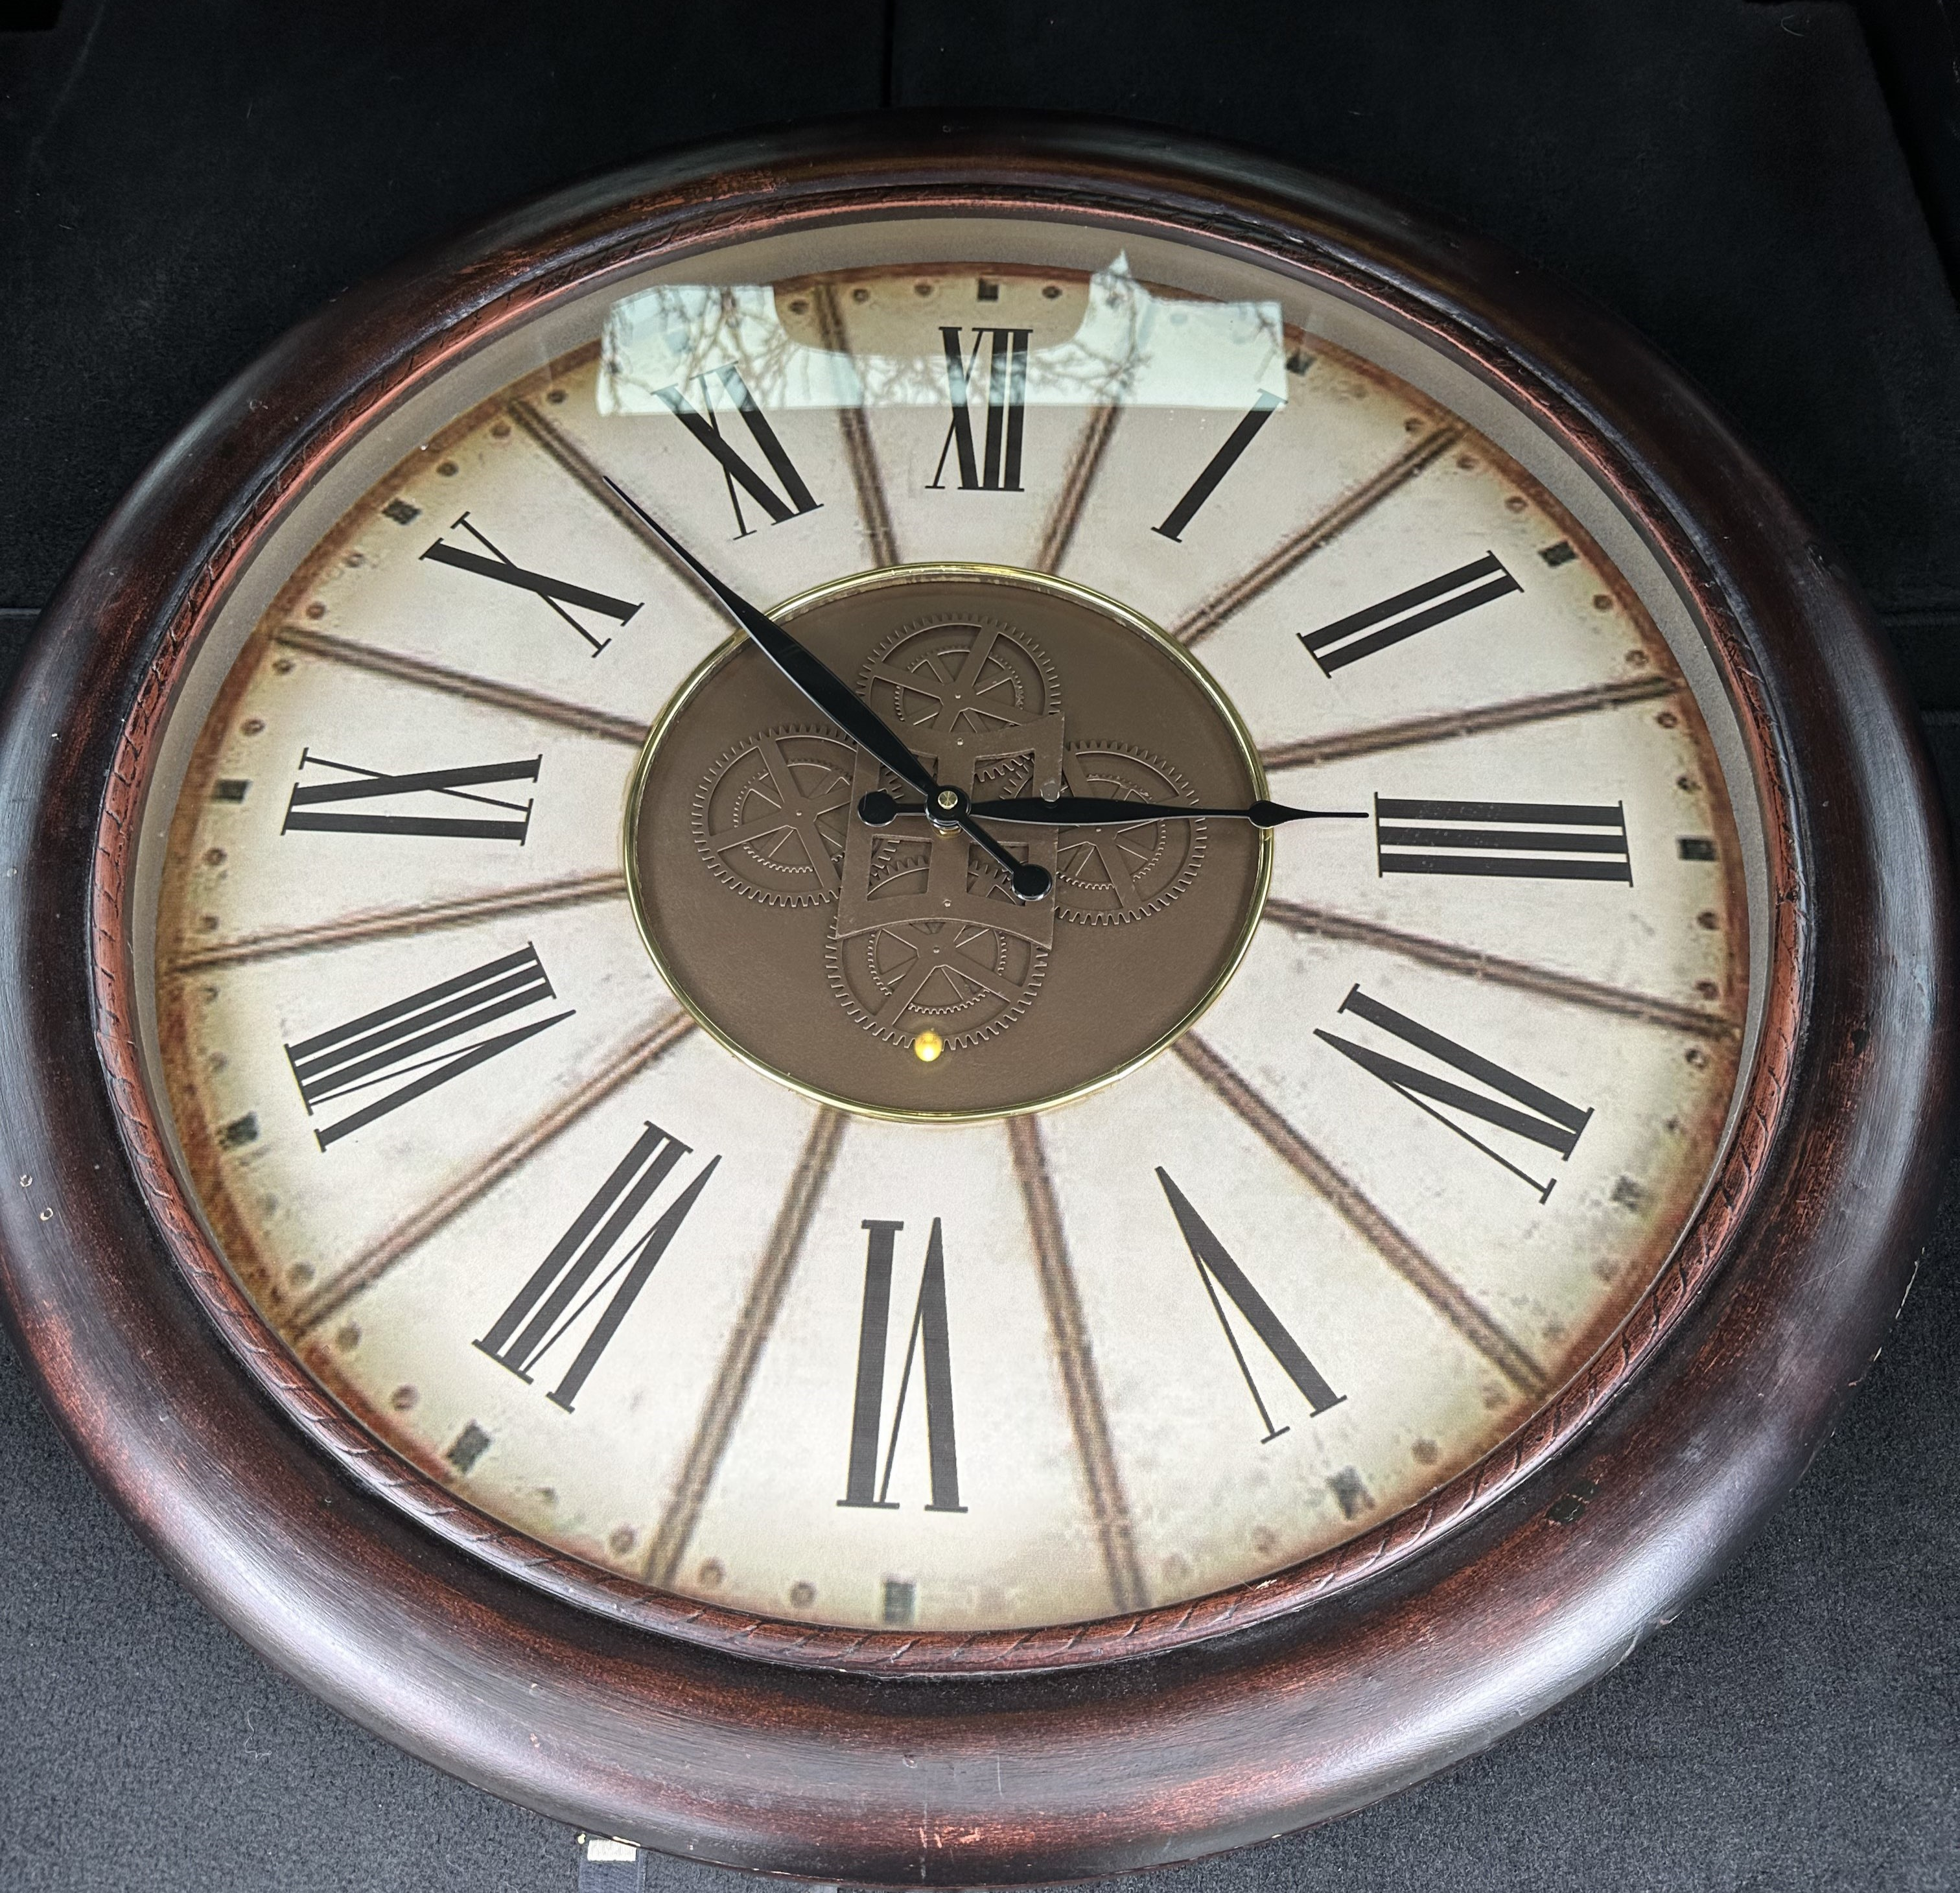
\includegraphics[width=0.85\columnwidth]{Images/big-clock.jpg}
    \caption{The big clock that we are using for the "Player Clock".}
\end{figure}


\section{Testing}
Different puzzles and modules of the game will be tested before combining
them all into what will become the escape room. Each module will have its
own specifications on what it should do. For example, the chess board puzzle
will have lots of different combinations tested just to make sure that only
the correct one will trigger a signal, which later will be the signal that
allows the players to leave the room. Modules will also be tested on
durability to make sure it is sturdy and not prone to easily breaking.
Players will be instructed to treat every object with care, so hopefully
the modules will not be tested of their strength outside of the testing
environment.
\\
\indent When each module is tested according to their specifications, and works
with small testing programs, then they will be combined into the bigger
room script of the game. From there, testing will be done for the room
as a whole to make sure that players are able to complete it. It may also
be necessary to bring in people unfamiliar with the game to try it out
themselves, that way feedback can be given of whether certain puzzles
need to be harder or easier. For the stretch goal, each possible combination
of puzzles would have to be tested to make sure there are no dead end routes.

\section{Demo}
The demo planned for this proposal is the clock that will be integral to
the puzzles in the escape room. Players must be expected to manipulate
this clock to activate certain events in the game, along with the clock
moving by itself throughout. Thus, a big analog clock will have controls
tied to it that either moves it forward in time or back in time. The
clock cannot go before 1:00 or past 12:00, and whatever time the clock
is at should be able to be read by a computer.
\\
\indent Likely, the analog clock will most likely just be a display to an internal
counter that counts on its own based on clock speed. By pressing either a
"forward" or "reverse" button, the counter will increment or decrement
and update the display on the clock alongside transferring the value to
a computer. This will make the time easily stored and tracked which will
help towards scripting certain events in the escape room.

\section{Conclusion}
Conclusion

\begin{thebibliography}{00}

    \bibitem{wikipediaEscapeRoom} “Escape room,” Wikipedia, 10-Feb-2023. [Online]. Available: \url{https://en.wikipedia.org/wiki/Escape_room}. [Accessed: 24-Mar-2023].
    \bibitem{whatIsAnEscapeRoom} A. Ascalon, “Escape rooms: Everything you need to know (2022),” Escape Rooms | Everything You Need To Know (2022), 01-Dec-2022. [Online]. Available:  \url{https://theescapegame.com/blog/what-is-an-escape-room/}. [Accessed: 24-Mar-2023].

\end{thebibliography}




\end{document}
